%
\documentclass[hyperref,handout,compress,9pt,mathserif]{beamer}
%\documentclass[hyperref,compress,9pt,mathserif]{beamer}

\usepackage{subfiles}
\usepackage{import}
\usepackage{listings}

% show presentation notes
\usepackage{pgfpages}
%\setbeameroption{show notes}
%\setbeameroption{show notes on second screen=right}

% a trick to allow subfiles to access the macro and definition files in the main folder
\makeatletter
\def\input@path{{./}{../}}
\makeatother

% let the main file read pictures in the subfolders
\graphicspath{{challenges/}{background/}{results/}{figs/}}

%% Version: 2013-11-26
%% common packages
\usepackage{hyperref}
\usepackage{amsbsy}
\usepackage{amsmath}
\usepackage{graphicx}
\usepackage{subfigure}
\usepackage{color}
\usepackage{multirow}
\usepackage{booktabs}
\usepackage{wasysym}
\usepackage{lmodern} % to avoid font size not available warning
\usepackage{textcomp} % to avoid font warning for textbullet used in \item
\usepackage{wasysym} % useful symbols
\usepackage{dashbox} % for use of dashd box \dbox{...}
\usepackage{mathtools} % for \DeclarePairedDelimiter below
\usepackage{tabto}  % for \NumTabs{3} and \tab commands
\usepackage[ruled,vlined]{algorithm2e}

%% to allow citation as footnote
\usepackage{natbib}
%  to reduce footnote font size
\usepackage{etoolbox}
\makeatletter
\patchcmd{\@makefntext}{\insertfootnotetext{#1}}{\insertfootnotetext{\scriptsize#1}}{}{}
\makeatother


%% macros for commenting
\usepackage[normalem]{ulem} % to use \sout
\newcommand{\remove}[1]{{\color{Gray}\sout{#1}}}
\newcommand{\revise}[1]{{\color{blue}#1}}
\newcommand{\commwy}[1]{{\color{red}(wy: #1)}} % Wotao Yin

%% template for beamer

\mode<presentation>
{
  % page number
  %\setbeamertemplate{footline}{\insertframenumber/\inserttotalframenumber}
  %\setbeamertemplate{footline}[frame number]

  % background and theme
  \setbeamertemplate{background canvas}[vertical shading][bottom=white!10,top=white!10]
  \usetheme{default}

  % section in table of contents has numbers
  \setbeamertemplate{sections/subsections in toc}[sections numbered]

  % no navigation bottoms
  \setbeamertemplate{navigation symbols}{}

  % itemize, black bullet, %150 spacing between items using "witemize"
  \setbeamertemplate{itemize items}[circle]
  \setbeamercolor{itemize item}{fg=black}
  \setbeamercolor{enumerate item}{fg=black}
  \setbeamercolor{itemize subitem}{fg=black}
  \setbeamercolor{enumerate subitem}{fg=black}
  \newenvironment{witemize}{\itemize\addtolength{\itemsep}{0.4\baselineskip}}{\enditemize}

  % itemize enumerate use normal sized texts
  \setbeamertemplate{itemize/enumerate body begin}{\normalsize}
  \setbeamertemplate{itemize/enumerate subbody begin}{\normalsize}
  \setbeamertemplate{itemize/enumerate subsubbody begin}{\normalsize}

  % block, black over gray with no shadow
  \setbeamertemplate{blocks}[rounded][shadow=false]
  \setbeamercolor{block title}{fg=black,bg=gray!40}
  \setbeamercolor{block body}{fg=black,bg=gray!10}

  % frametitle, bold, black, centered
  \setbeamertemplate{frametitle}[default][center]
  \setbeamercolor{frametitle}{fg=black}
  \setbeamerfont{frametitle}{shape=\bfseries}

  % line spacing
  \linespread{1.2}

  \setlength{\parskip}{\smallskipamount}
}

% use \beginbackup ... \backupend for backup slides, from fuenfundachtzig on stackoverflow.com
\newcommand{\backupslidesbegin}{
   \newcounter{framenumbervorappendix}
   \setcounter{framenumbervorappendix}{\value{framenumber}}
}
\newcommand{\backupslidesend}{
   \addtocounter{framenumbervorappendix}{-\value{framenumber}}
   \addtocounter{framenumber}{\value{framenumbervorappendix}}
}

%% macros for letters

\newcommand{\va}{{\mathbf{a}}}
\newcommand{\vb}{{\mathbf{b}}}
\newcommand{\vc}{{\mathbf{c}}}
\newcommand{\vd}{{\mathbf{d}}}
\newcommand{\ve}{{\mathbf{e}}}
\newcommand{\vf}{{\mathbf{f}}}
\newcommand{\vg}{{\mathbf{g}}}
\newcommand{\vh}{{\mathbf{h}}}
\newcommand{\vi}{{\mathbf{i}}}
\newcommand{\vj}{{\mathbf{j}}}
\newcommand{\vk}{{\mathbf{k}}}
\newcommand{\vl}{{\mathbf{l}}}
\newcommand{\vm}{{\mathbf{m}}}
\newcommand{\vn}{{\mathbf{n}}}
\newcommand{\vo}{{\mathbf{o}}}
\newcommand{\vp}{{\mathbf{p}}}
\newcommand{\vq}{{\mathbf{q}}}
\newcommand{\vr}{{\mathbf{r}}}
\newcommand{\vs}{{\mathbf{s}}}
\newcommand{\vt}{{\mathbf{t}}}
\newcommand{\vu}{{\mathbf{u}}}
\newcommand{\vv}{{\mathbf{v}}}
\newcommand{\vw}{{\mathbf{w}}}
\newcommand{\vx}{{\mathbf{x}}}
\newcommand{\vy}{{\mathbf{y}}}
\newcommand{\vz}{{\mathbf{z}}}

\newcommand{\vA}{{\mathbf{A}}}
\newcommand{\vB}{{\mathbf{B}}}
\newcommand{\vC}{{\mathbf{C}}}
\newcommand{\vD}{{\mathbf{D}}}
\newcommand{\vE}{{\mathbf{E}}}
\newcommand{\vF}{{\mathbf{F}}}
\newcommand{\vG}{{\mathbf{G}}}
\newcommand{\vH}{{\mathbf{H}}}
\newcommand{\vI}{{\mathbf{I}}}
\newcommand{\vJ}{{\mathbf{J}}}
\newcommand{\vK}{{\mathbf{K}}}
\newcommand{\vL}{{\mathbf{L}}}
\newcommand{\vM}{{\mathbf{M}}}
\newcommand{\vN}{{\mathbf{N}}}
\newcommand{\vO}{{\mathbf{O}}}
\newcommand{\vP}{{\mathbf{P}}}
\newcommand{\vQ}{{\mathbf{Q}}}
\newcommand{\vR}{{\mathbf{R}}}
\newcommand{\vS}{{\mathbf{S}}}
\newcommand{\vT}{{\mathbf{T}}}
\newcommand{\vU}{{\mathbf{U}}}
\newcommand{\vV}{{\mathbf{V}}}
\newcommand{\vW}{{\mathbf{W}}}
\newcommand{\vX}{{\mathbf{X}}}
\newcommand{\vY}{{\mathbf{Y}}}
\newcommand{\vZ}{{\mathbf{Z}}}

\newcommand{\cA}{{\mathcal{A}}}
\newcommand{\cB}{{\mathcal{B}}}
\newcommand{\cC}{{\mathcal{C}}}
\newcommand{\cD}{{\mathcal{D}}}
\newcommand{\cE}{{\mathcal{E}}}
\newcommand{\cF}{{\mathcal{F}}}
\newcommand{\cG}{{\mathcal{G}}}
\newcommand{\cH}{{\mathcal{H}}}
\newcommand{\cI}{{\mathcal{I}}}
\newcommand{\cJ}{{\mathcal{J}}}
\newcommand{\cK}{{\mathcal{K}}}
\newcommand{\cL}{{\mathcal{L}}}
\newcommand{\cM}{{\mathcal{M}}}
\newcommand{\cN}{{\mathcal{N}}}
\newcommand{\cO}{{\mathcal{O}}}
\newcommand{\cP}{{\mathcal{P}}}
\newcommand{\cQ}{{\mathcal{Q}}}
\newcommand{\cR}{{\mathcal{R}}}
\newcommand{\cS}{{\mathcal{S}}}
\newcommand{\cT}{{\mathcal{T}}}
\newcommand{\cU}{{\mathcal{U}}}
\newcommand{\cV}{{\mathcal{V}}}
\newcommand{\cW}{{\mathcal{W}}}
\newcommand{\cX}{{\mathcal{X}}}
\newcommand{\cY}{{\mathcal{Y}}}
\newcommand{\cZ}{{\mathcal{Z}}}

\newcommand{\ba}{{\boldsymbol{a}}}
\newcommand{\bb}{{\boldsymbol{b}}}
\newcommand{\bc}{{\boldsymbol{c}}}
\newcommand{\bd}{{\boldsymbol{d}}}
\newcommand{\be}{{\boldsymbol{e}}}
\renewcommand{\bf}{{\boldsymbol{f}}}
\newcommand{\bg}{{\boldsymbol{g}}}
\newcommand{\bh}{{\boldsymbol{h}}}
\newcommand{\bi}{{\boldsymbol{i}}}
\newcommand{\bj}{{\boldsymbol{j}}}
\newcommand{\bk}{{\boldsymbol{k}}}
\newcommand{\bl}{{\boldsymbol{l}}}
\newcommand{\bm}{{\boldsymbol{m}}}
\newcommand{\bn}{{\boldsymbol{n}}}
\newcommand{\bo}{{\boldsymbol{o}}}
\newcommand{\bp}{{\boldsymbol{p}}}
\newcommand{\bq}{{\boldsymbol{q}}}
\newcommand{\br}{{\boldsymbol{r}}}
\newcommand{\bs}{{\boldsymbol{s}}}
\newcommand{\bt}{{\boldsymbol{t}}}
\newcommand{\bu}{{\boldsymbol{u}}}
\newcommand{\bv}{{\boldsymbol{v}}}
\newcommand{\bw}{{\boldsymbol{w}}}
\newcommand{\bx}{{\boldsymbol{x}}}
\newcommand{\by}{{\boldsymbol{y}}}
\newcommand{\bz}{{\boldsymbol{z}}}

\newcommand{\bA}{{\boldsymbol{A}}}
\newcommand{\bB}{{\boldsymbol{B}}}
\newcommand{\bC}{{\boldsymbol{C}}}
\newcommand{\bD}{{\boldsymbol{D}}}
\newcommand{\bE}{{\boldsymbol{E}}}
\newcommand{\bF}{{\boldsymbol{F}}}
\newcommand{\bG}{{\boldsymbol{G}}}
\newcommand{\bH}{{\boldsymbol{H}}}
\newcommand{\bI}{{\boldsymbol{I}}}
\newcommand{\bJ}{{\boldsymbol{J}}}
\newcommand{\bK}{{\boldsymbol{K}}}
\newcommand{\bL}{{\boldsymbol{L}}}
\newcommand{\bM}{{\boldsymbol{M}}}
\newcommand{\bN}{{\boldsymbol{N}}}
\newcommand{\bO}{{\boldsymbol{O}}}
\newcommand{\bP}{{\boldsymbol{P}}}
\newcommand{\bQ}{{\boldsymbol{Q}}}
\newcommand{\bR}{{\boldsymbol{R}}}
\newcommand{\bS}{{\boldsymbol{S}}}
\newcommand{\bT}{{\boldsymbol{T}}}
\newcommand{\bU}{{\boldsymbol{U}}}
\newcommand{\bV}{{\boldsymbol{V}}}
\newcommand{\bW}{{\boldsymbol{W}}}
\newcommand{\bX}{{\boldsymbol{X}}}
\newcommand{\bY}{{\boldsymbol{Y}}}
\newcommand{\bZ}{{\boldsymbol{Z}}}

\newcommand{\ri}{{\mathrm{i}}}
\newcommand{\rr}{{\mathrm{r}}}

%% macros for math notions and operators

\newcommand{\RR}{\mathbb{R}}
\newcommand{\CC}{\mathbb{C}}
\newcommand{\ZZ}{\mathbb{Z}}
\renewcommand{\SS}{{\mathbb{S}}}
\newcommand{\SSp}{\mathbb{S}_{+}}
\newcommand{\SSpp}{\mathbb{S}_{++}}
\newcommand{\sign}{\mathrm{sign}}
\newcommand{\Sign}{\mathrm{Sign}}
\newcommand{\vzero}{\mathbf{0}}
\newcommand{\vone}{{\mathbf{1}}}
\newcommand{\Null}{{\mathrm{Null}}}
\newcommand{\dist}{{\mathrm{dist}}}
\newcommand{\Co}{{\mathbf{Co}}}

\newcommand{\op}{{\mathrm{op}}} % subscript for operator norm
\newcommand{\opt}{{\mathrm{opt}}} % subscript for optimal solution
\newcommand{\supp}{{\mathrm{supp}}} % support
\newcommand{\Prob}{{\mathrm{Prob}}} % probability
\newcommand{\Diag}{{\mathrm{Diag}}} % vector -> diagonal matrix
\newcommand{\diag}{{\mathrm{diag}}} % matrix diagonal -> vector
\newcommand{\dom}{{\mathrm{dom}}} % domain
\newcommand{\grad}{{\nabla}}    % gradient
\newcommand{\tr}{{\mathrm{tr}}} % trace
\newcommand{\TV}{{\mathrm{TV}}} % total variation
\newcommand{\Proj}{{\mathrm{Proj}}}
\DeclareMathOperator{\shrink}{shrink} % shrinkage
\DeclareMathOperator*{\argmin}{arg\,min}
\DeclareMathOperator*{\argmax}{arg\,max}
\DeclareMathOperator*{\mini}{minimize}
\DeclareMathOperator*{\maxi}{maximize}
\DeclareMathOperator*{\Min}{minimize}
\DeclareMathOperator*{\Max}{maximize}
\newcommand{\fwd}{{\mathbf{fwd}}}
\newcommand{\prox}{{\mathbf{prox}}}
\newcommand{\refl}{{\mathbf{refl}}}
\newcommand{\proj}{{\mathbf{proj}}}
\newcommand{\solve}{\stackrel{\mathrm{solve}}\longleftarrow}
\newcommand{\st}{{\quad\mathrm{s.t.}}}
\newcommand{\St}{{\quad\mathrm{subject~to}}}
\newcommand{\pt}{{\textbullet\ }}

% --- OpSplitting specific macro ---
\newcommand{\Fix}{{\mathrm{Fix}}}
\newcommand{\tnabla}{{\widetilde{\nabla}}}
\newcommand{\TFBS}{T_{\mathrm{FBS}}}
\newcommand{\TBFS}{T_{\mathrm{BFS}}}
\newcommand{\TFBFS}{T_{\mathrm{FBFS}}}
\newcommand{\TPRS}{T_{\mathrm{PRS}}}
\newcommand{\TDRS}{T_{\mathrm{DRS}}}
\newcommand{\TPRSl}{T^\lambda_{\mathrm{PRS}}}
\newcommand{\kbest}{k_{\mathrm{best}}}

\DeclarePairedDelimiter{\ceil}{\lceil}{\rceil}
\DeclarePairedDelimiter{\floor}{\lfloor}{\rfloor}
\DeclarePairedDelimiter{\dotp}{\langle}{\rangle}

%% macros for environments math equations

\newcommand{\MyFigure}[1]{../fig/#1}

\newcommand{\bdm}{\begin{displaymath}}
\newcommand{\edm}{\end{displaymath}}

\newcommand{\beq}{\begin{equation}}
\newcommand{\eeq}{\end{equation}}

\newcommand{\bfl}{\begin{flushleft}}
\newcommand{\efl}{\end{flushleft}}

\newcommand{\beqn}{\begin{eqnarray}}
\newcommand{\eeqn}{\end{eqnarray}}

\newcommand{\beqs}{\begin{align*}} % no equation numbers
\newcommand{\eeqs}{\end{align*}}  % no equation numbers

%% macros for theorem-like environments

%\newtheorem{theorem}{Theorem}
\newtheorem{condition}{Condition}
\newtheorem{assumption}{Assumption}
%\newtheorem{definition}{Definition}
%\newtheorem{corollary}{Corollary}
%\newtheorem{remark}{Remark}
%\newtheorem{lemma}{Lemma}
%\newtheorem{proof}{Proof}
\newtheorem{proposition}{Proposition}
%\newtheorem{example}{Example}

%\newtheorem{example}[remark]{Example}
 % --- take a look at this macro file ---

\usepackage{xcolor}
\usepackage{hyperref}

\hypersetup{%
  colorlinks=false,% hyperlinks will be black
  linkbordercolor=red,% hyperlink borders will be red
  pdfborderstyle={/S/U/W 1}% border style will be underline of width 1pt
}



% --- drawing ---
\usepackage{tikz}
\usetikzlibrary{positioning}
\usetikzlibrary{shadows}

% --- blue equation box ---
\usepackage{empheq}
\definecolor{myblue}{rgb}{.8, .8, 1}
\newcommand*\mybluebox[1]{%
\colorbox{myblue}{\hspace{1em}#1\hspace{1em}}}

% --- to include codes ---
\usepackage{listings}
\lstset{language=C++,
                basicstyle=\ttfamily,
                keywordstyle=\color{blue}\ttfamily,
                stringstyle=\color{blue}\ttfamily,
                commentstyle=\color{red}\ttfamily,
                morecomment=[l][\color{blue}]{\#},
                backgroundcolor=\color{black!5} % set backgroundcolor
}

\AtBeginSection[]
{
  \begin{frame}<beamer>
    \frametitle{Outline for section \thesection}
    \tableofcontents[currentsection]
  \end{frame}
}



\begin{document}

\title{The Guide of the MOTAC Codebase}
% \author{Zhimin Peng %(UCLA Math)%\\ Rice CAAM (by courtesy)
% }
%
%\institute{
%\begin{normalsize}
%  Joint work with {Brent Edmunds, Yezheng Li, Yerong Li, Yangyang Xu,  Ming Yan, Wotao Yin}
%\end{normalsize}
%}

\date{
  \today
}


\begin{frame}
  \titlepage
\end{frame}


\section{Background}
\begin{frame}\begin{center}\begin{Large}\textbf{Background}\end{Large}\end{center}\end{frame}

\begin{frame}{The fixed-point problem}
\begin{witemize}
\item operator $T: \cH \rightarrow \cH$
\item \textbf{problem:} find $x\in\cH$ such that
$$x = Tx$$\pause
\note[item]{The underlying problem is abstracted to finding a fixed point to a nonexpansive operator $T$, which is assumed to have a fixed point. In fact, the condition can be relaxed to: there exists $\mu>0$ such that $I-\mu(I-T)$ is nonexpansive.}
%\item equivalently, let $S:=I-T$, find $x\in\cH$ such that
%$$0= Sx$$\pause
%\item Operator $T:\cH\to\cH$, where $\cH$ is a Hilbert space and $T$ satisfies
% $$\|Tx-Ty\|\le \|x-y\|,\quad \forall x,y\in \cH$$
  \note[item]{Our setting is a (possibly infinite dimensional) Hilbert space.}
  \note[item]{We will use $S$ instead of $T$ to develop our algorithm.}
\item abstracts many problems:
\begin{itemize}
\item linear equations
\item convex optimization
\item statistical regression
\item optimal control
\end{itemize}
\end{witemize}
\end{frame}

\begin{frame}{MOTAC\footnote{Peng-Xu-Yan-Y.'15}: Async-parallel coordinate update}

\begin{itemize}
  \item $\cH = \cH_1 \times \cdots \times \cH_m$
  \item $p$ agents, possibly $p\not=m$
  \item each agent {randomly picks} $i\in\{1,\ldots,m\}$ and updates just $x_i$:
\begin{align*}
x_1^{k+1}&\gets x_1^k\\
&\vdots\\
%x_{i-1}^{k+1}&\gets x_{i-1}^k\\
x_i^{k+1}&\gets x_i^k - \eta_k S_i {\hat{x}^k}\\
%x_{i+1}^{k+1}&\gets x_{i+1}^k\\
&\vdots\\
x_{m}^{k+1}&\gets x_{m}^k
\end{align*}
where $S = I - T$.
\end{itemize}
\end{frame}

\begin{frame}{What's wrong with the old code?}
\begin{itemize}
\item It is cluttered;
\item It is not portable;
\item Creating a new app is troublesome.
\end{itemize}
\end{frame}

\begin{frame}{The goal of the new code base}
\begin{itemize}
\item Be able to create a new app quickly;
\item Be able to test new asynchronous ideas easily;
\item Be portable and modularized;
\item Academic friendly;
\end{itemize}
\end{frame}

\begin{frame}{Features}
\begin{itemize}
\item Vector and matrix classes (both dense and sparse);
\item A customized and easy-to-use linear algebra library; 
\item A rich set of coordinate friendly operators (\textbf{17} operators);
\item Several interfaces for common operator splitting schemes; 
\item A rich set of applications built on top of MOTAC;
\item A generic interface for controller;
\item Matlab, Python and Julia interface (coming soon);
\item Runs on Linux, Mac OS X and Windows;
\item Approximately 5,000 lines of C++ source code.
\end{itemize}
\end{frame}

\section{The Architecture}
\begin{frame}\begin{center}\begin{Large}\textbf{Architecture}\end{Large}\end{center}\end{frame}

\begin{frame}
\begin{figure}[!h]
        \centering
                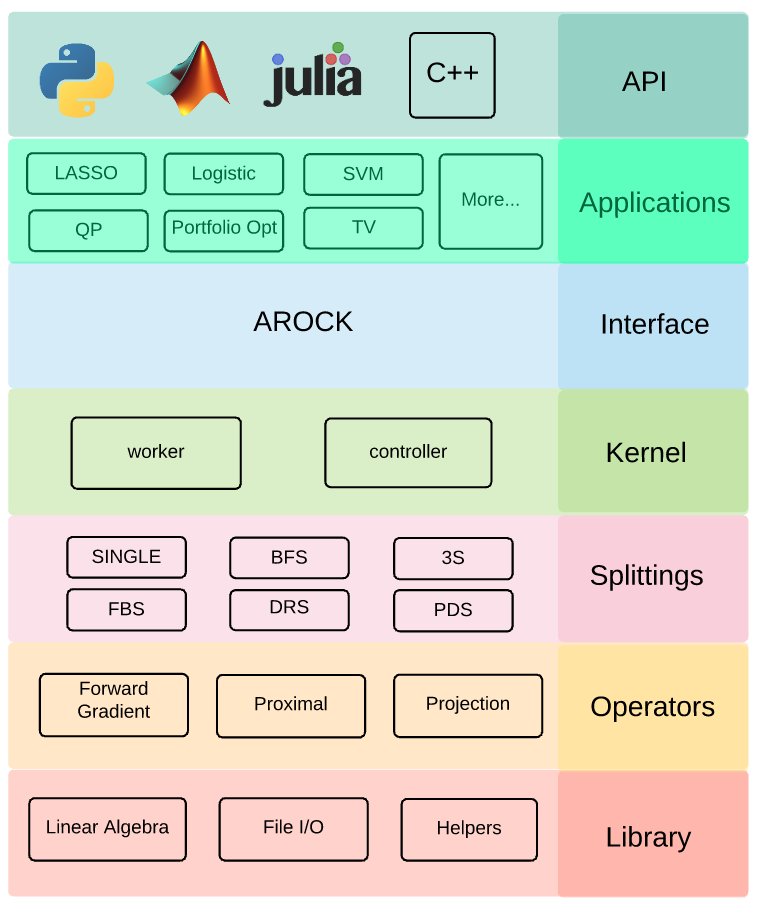
\includegraphics[width=0.72\textwidth]{./figs/architecture}
\end{figure}
\end{frame}

\begin{frame}{Library}
Matrix and Vector
\begin{itemize}
\item We use the sparse matrix and sparse vector classes from \texttt{Eigen};
\item We build our own dense matrix and dense vector classes based on \texttt{std::vector};
\end{itemize}

Linear Algebra
\begin{itemize}
\item Naive implementation is under the \texttt{MyAlgebra} namespace;
\item Interface for \texttt{BLAS} is under the \texttt{BLASAlgebra} namespace;
\end{itemize}

File I/O
\begin{itemize}
\item Matrix market format;
\item LIBSVM format;
\item Matlab format (coming soon)
\end{itemize}

Helpers
\begin{itemize}
\item Objective function;
\item Input args parser;
\end{itemize}
\end{frame}

\begin{frame}[fragile]{Operator - template}
\begin{small}
\begin{lstlisting}
 struct functor_name {                                                                                                                                                           
   // the step_size that associated with the operator                                                                                                                            
   double step_size;                                                                                                                                                             
   // weight on the original function                                                                                                    
   double weight;                                                                                                                                                                                                                                                                                                                                                 
   // returns the operator evaluated on v at the given index                                                                                                                       
   double operator() (Vector* v, int index);                                                                                                                                                            
   // returns the operator evaluated on val at the given index                                                                                                                       
   double operator() (double val, int index);                                                                                                               
   // full update                                                                                                                                                                          
   void operator() (Vector* v_in, Vector* v_out);
   // (Optional) update the cached variables                                                                                                                                   
   void update_cache_vars (double old_x_i, double new_x_i, 
                                       int index);                                                                                                                                                                                
   // update the step size                                                                                                                               
   void update_step_size (double step_size_); 
   // customized constructor                                                                                                                                                                             
   functor_name (double step_size_, double weight_ = 1.);
   // default constructor                                                                                                                                                          
   functor_name () : step_size(0.), weight(1.) {}                                                                                                                                                                                                                                                                                                     
};                                                                                                                                                                                
\end{lstlisting}
\end{small}
\end{frame}



\begin{frame}{Operator - Proximal}
$$\prox_f (x) = \argmin_{y} f(y) + \frac{1}{2\sigma} \|x - y\|^2$$
\begin{small}

\begin{table}[htbp]
\centering
 \begin{tabular}{|c|c|c|}
  \hline
  Name & Definition & Proximal operator \\
  \hline
  \hline
  $\ell_1$ norm & $w \|x\|_1$ & $shrink(x, w \cdot \sigma)$ \\
  \hline  
  sum of squares & $\frac{w}{2} \|x\|_2^2$ & $\frac{1}{1 + w \cdot \sigma} x$ \\
  \hline 
  $\ell_2$ norm & $w \|x\|_2$ & $\begin{cases} 
  							0 & \text{ if } \|x\|_2 \leq w \sigma \\
							(1 - \frac{w \sigma}{\|x\|_2}) \cdot x & \text{otherwise}
							\end{cases}$ \\							
  \hline
  Huber function & $ \begin{cases}
  				\frac{w}{2} x^2, &\text{if} -\delta \leq x \leq \delta \\
				 w \delta(|x| - \frac{\delta}{2}), &\text{otherwise} \\
  			       \end{cases}$ & $\begin{cases} x -  w \sigma  \delta & \text{ if } x \geq \delta +  w \sigma \delta\\
			       \frac{x}{1 + \sigma w} & \text{ otherwise } \\
			        x +  w \sigma \delta  & \text{ if } x \leq -\delta -  w \sigma \delta\\
			       \end{cases}$ \\
  \hline		
 elastic net & $w_1 \|x\|_1 + \frac{w_2}{2} \|x\|_2^2$ &  $\frac{1}{1 + w_2 \sigma} \cdot shrink(x, w_1 \sigma)$\\
 \hline
 log barrier & $- w \sum_{i} \log(x_i)$ & $\frac{1}{2} (x_i + \sqrt{x_i^2 + 4 w \sigma}), \forall i$ \\
 \hline
 \end{tabular}
\end{table}
\end{small}
\end{frame}


\begin{frame}{Operator - Projections}
\begin{small}
\begin{table}[htbp]
\centering
 \begin{tabular}{|c|c|c|}
  \hline
  Name & Definition & Projection operator \\
  \hline
  \hline
  positive cone & $\{x ~|~ x \geq 0\}$ & $\max(0, x_i), \forall i$ \\
  \hline
  box & $\{x ~|~ l \leq x \leq u\}, l, u \in R^n$ & $\max(l_i, \min(x_i, u_i))$ \\
  \hline
  $\ell_1$ ball & $\{ x ~|~ \|x\|_1 \leq r \}$ & $O(n\log(n))$ method\\
  \hline 
  $\ell_2$ ball & $\{ x ~|~ \|x\|_2 \leq r \}$ & $\begin{cases} \frac{r}{\|x\|} \cdot x ~&\text{ if } \|x\|_2 \geq r \\
  										         x ~&\text{ otherwise }
  								   \end{cases} $\\
  \hline 
  hyperplane & $\{ x ~|~ a^T x = b \}$ & $x + \frac{(b - a^T x)}{a^Ta} \cdot a$\\
  \hline 
  probability simplex & $\{ x ~|~  x \geq 0, \sum_i x_i = 1\}$ & $O(n\log(n))$ method\\
  \hline   
 \end{tabular}
\end{table}
\end{small}
\end{frame}

\begin{frame}{Operator - Forward gradient}
\begin{small}
\begin{table}[htbp]
\hspace*{-3em}
 \begin{tabular}{|c|c|c|}
  \hline
  Name & Definition & Forward gradient operator \\
  \hline
  \hline
  square loss & $\frac{w}{2}\|A^Tx - b\|^2$ & $x - \sigma w A (A^T x - b)$ \\
  \hline
  quadratic function & $w (\frac{1}{2} x^T Q x + c^Tx + d)$ & $x - \sigma w (Q x + c)$ \\
  \hline
  logistic loss & $w \sum_i \log (1 + \exp(- b_i \cdot a_i^T x)) $ &  $x + \sigma w \sum_i \frac{b_i}{1 + \exp(b_i \cdot a_i^T x)} \cdot a_i$\\
  \hline
   square hinge loss & $\frac{w}{2} \sum \max(0, b_i (1 - a_i^T x))^2$ & $x +  \sigma w\sum b_i \max(0, b_i (1 - a_i^T x)) \cdot a_i$ \\
  \hline
   square huber loss & $w \sum huber(a_i^Tx - b_i)$ & $x  - \sigma  w \nabla huber(a_i^T x - b_i)$ \\
  \hline
 \end{tabular}
\end{table}
\end{small}
Other loss functions:
\begin{itemize}
\item error functions in neural networks (coming soon);
\end{itemize}
\end{frame}


\begin{frame}{Splitting schemes}
Splitting schemes templated on one or more than one operators. The following are the supported splitting schemes:
\begin{itemize}
\item proximal point algorithm;
\item forward gradient algorithm;
\item forward-backward splitting;
\item backward-forward splitting;
\item Peaceman-Rachford splitting;
\item three operator splitting; (coming soon)
\item primal-dual splitting; (coming soon)
\end{itemize}
\end{frame}

\begin{frame}[fragile]{Splitting schemes - example}
\begin{small}
\begin{lstlisting}
template <typename Forward, typename Backward>                                                                                                                                       
struct ForwardBackwardSplitting {                                                                                                                                                    
  Forward forward;                                                                                                                                                                   
  Backward backward;                                                                                                                                                                 
  Vector* x;                                                                                                                                                                         
  double relaxation_step_size;                                                                                                                                                       
  // constructor                                                                                                                                                                                   
  ForwardBackwardSplitting(Vector*, Forward, Backward);
  // update parameters                                                                                                                                                                                   
  void update_params(Params* params) {                                                                                                                                               
    forward.update_step_size(params->get_step_size());                                                                                                                               
    backward.update_step_size(params->get_step_size());                                                                                                                              
    relaxation_step_size = params->get_motac_step_size();                                                                                                                            
  }                                                                                                                                                                                  
  // make update to x[index], and update the cached variables                                                                                                                                                                                   
  double operator() (int index);                                                                                                                                          
};                                                                                                                                                                                   
\end{lstlisting}
\end{small}

\end{frame}


\begin{frame}{The two roles: worker and controller}
\begin{figure}[!h]
        \centering
                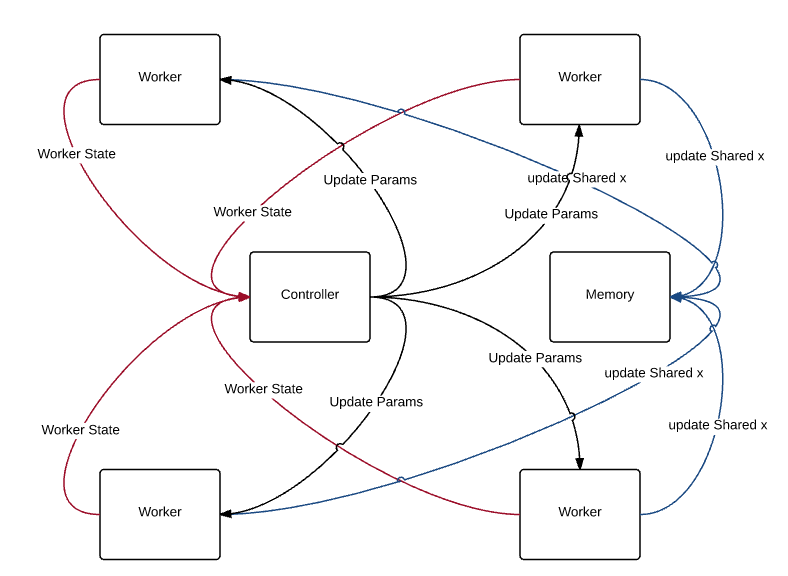
\includegraphics[width=.95\textwidth]{./figs/shared_arch.png}
\end{figure}
\end{frame}

\begin{frame}[fragile]{Worker}
Worker takes a splitting scheme, and a range of indexes, then runs \texttt{params->max\_itrs} of epochs. Other updating orders can be achieved through modifying the \texttt{worker} and the \texttt{AROCK} kernel.
\begin{lstlisting}
template<typename Splitting>
void worker(Splitting algorithm, 
	            Range range, 
	            Controller<Splitting>& cont, 
	            Params* params);
\end{lstlisting}

\end{frame}

\begin{frame}{Controller}
\begin{itemize}
\item controller object: defines the interaction between controller and worker. 
\item controller loop: update FPR and dynamically update the step size. 
% \item the flow chat is \href{https://www.lucidchart.com/invitations/accept/f18e1fc4-e5c7-4e39-804b-af012d483c4b}{here}.
\end{itemize}
\end{frame}

\begin{frame}{MOTAC}
Spawn a set of threads to execute the worker function and the controller loop function. 

\end{frame}



\begin{frame}{Implemented applications}
\begin{enumerate}
\begin{small}
\item find the intersection of two sets with PRS
$$\min_{x} \iota_{\{x| \|x\|_2 \leq 1\}} + \iota_{\{x | \|x\|_{\infty} \leq 0.1\}}$$
\item gradient descent for least squares
$$\min_{x} \frac{1}{2} \|A^Tx - b\|^2$$
\item FBS for LASSO
$$\min_{x} \lambda \|x\|_1 + \frac{1}{2} \|A^Tx - b\|^2$$
\item generalized regularized logistic regression
$$\min_{x} \lambda_1 \|x\|_1 + \frac{\lambda_{2}}{2} \|x\|^2 + \sum_{i = 1}^m \log(1 + \exp(-b_i \cdot a_i^T x))$$
\item BFS for simple quadratic constrained quadratic programming 
$$\min \frac{1}{2} \|A^Tx - b\|^2, \text{ s.t. } \|x\| \leq 1$$
\item FBS for modified version of SVM (coming soon)
$$ \min_{x} \frac{\lambda}{2} \|x\|^2 + \sum_{i=1}^m \max(0, 1 - b_i \cdot a_i^T x)^2  $$
\end{small}
\end{enumerate}
\end{frame}




\section{Numerical Tests}
\begin{frame}\begin{center}\begin{Large}\textbf{Numerical}\end{Large}\end{center}\end{frame}

\begin{frame} {Platform}
\begin{itemize}
\item a node with two Intel Xeon Processors E5-2690 v2 (25M Cache, 3.00 GHz)
\item 20 cores, 64 GB of RAM;
\end{itemize}


\end{frame}


\begin{frame}{Speedup test - baseline tests}
\begin{itemize}
\item Goal: test the speedup performance of a set of basic operations;
\item They will serve as a performance guideline for applying MOTAC to different applications;
\item We implemented the following tests:
\begin{itemize}
\item dot product of two dense vectors;
\item evaluate $\log(1 + \exp(-5.))$;
\item calculate $\text{dot}(A(i, :), x)$ for dense $A$;
\item calculate $\text{dot}(A(i, :), x)$ for sparse $A$; 

\end{itemize}
\end{itemize}

\end{frame}

\begin{frame}{Speedup test - dot product of two dense vectors}
\begin{itemize}
\item evaluate $x^T y$ for 3200 times.
\end{itemize}


\begin{figure}[!h]
        \centering
                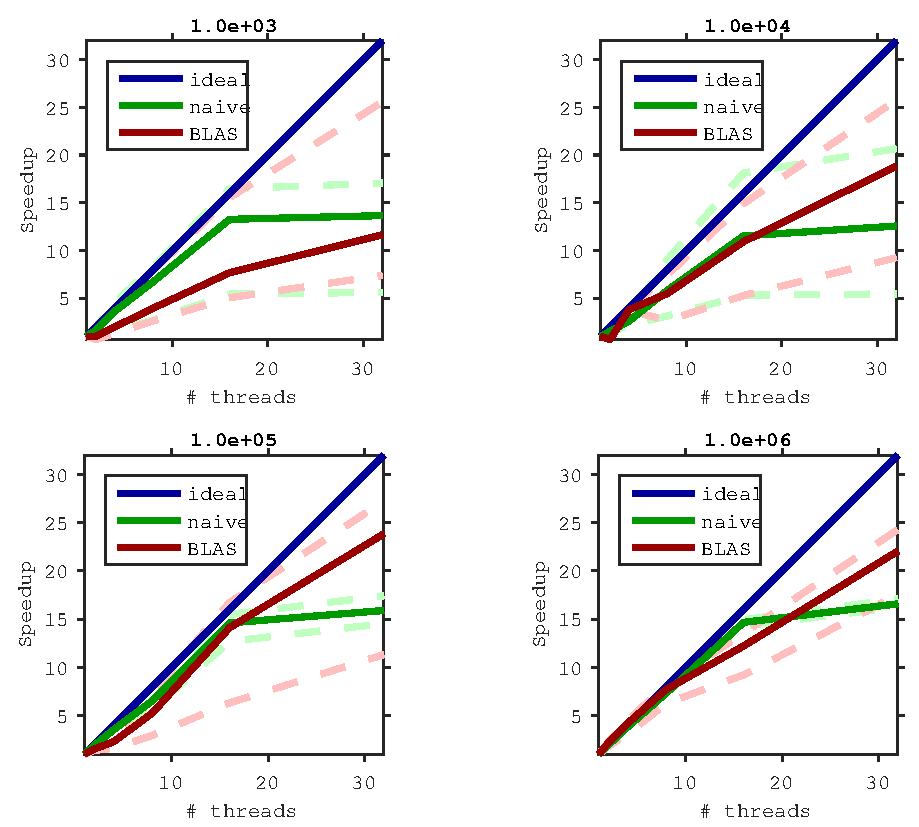
\includegraphics[width=.8\textwidth]{./figs/ds_vec_dot_prod_cropped.pdf}
\end{figure}

\end{frame}


\begin{frame}{Speedup test - evaluate logistic loss function}
\begin{itemize}
\item evaluate $\log(1 + \exp(-8.8))$ for 32 million times.
\end{itemize}

\begin{figure}[!h]
        \centering
                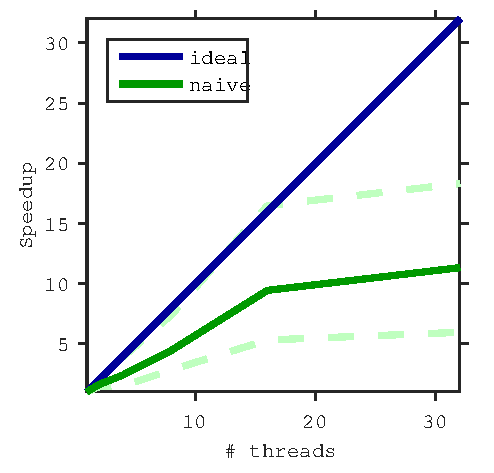
\includegraphics[width=.5\textwidth]{./figs/log_loss_cropped.pdf}
\end{figure}
\end{frame}


\begin{frame}{Speedup test - calculate $\text{dot}(A(i, :), x)$ for dense $A$;}
\begin{figure}[!h]
        \centering
                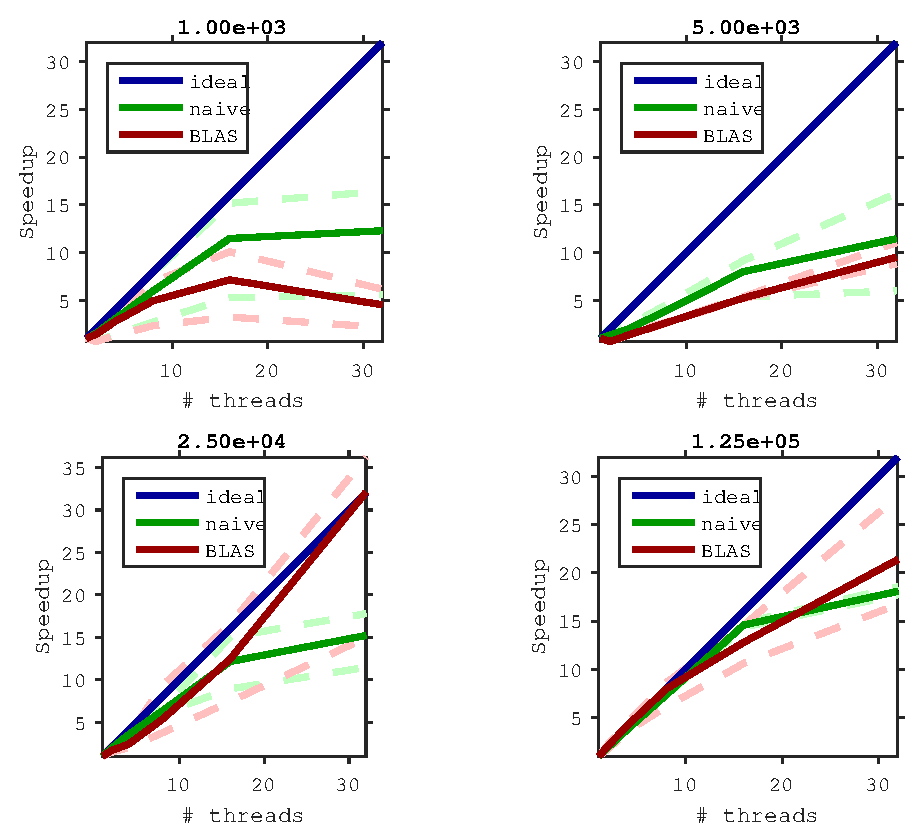
\includegraphics[width=.8\textwidth]{./figs/ds_matrix_ds_vec_speedup_cropped.pdf}
\end{figure}
\end{frame}


\begin{frame}{Speedup test - calculate $\text{dot}(A(i, :), x)$ for dense $A$;}
\begin{figure}[!h]
        \centering
                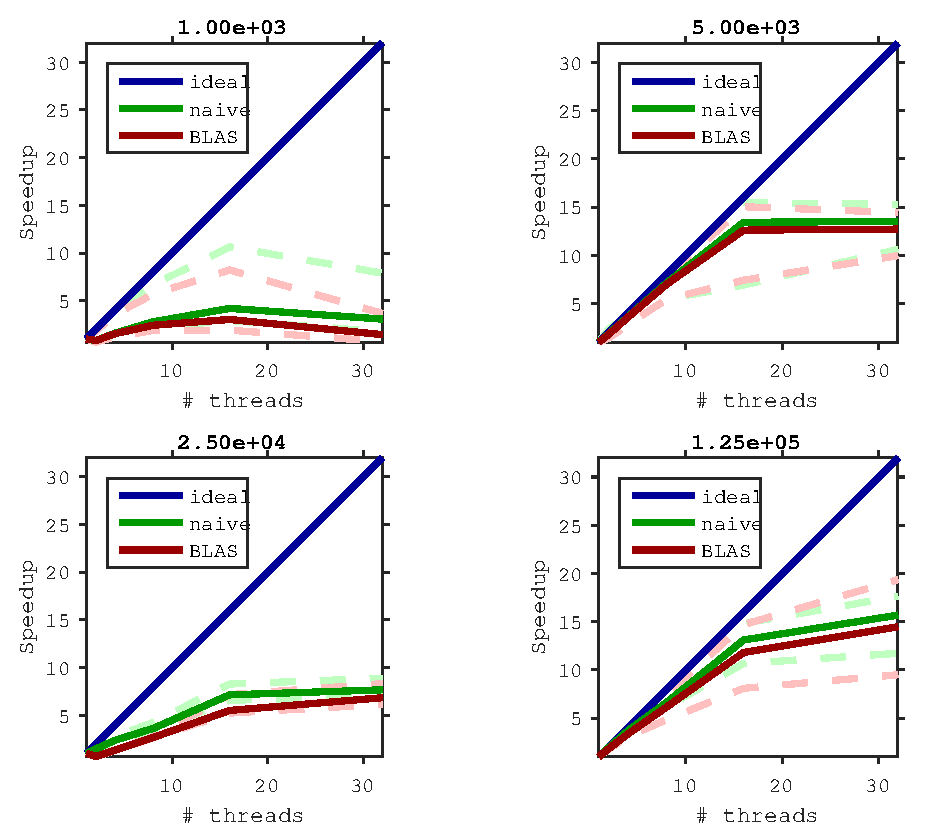
\includegraphics[width=.8\textwidth]{./figs/sp_mtx_ds_vec_speedup_cropped.pdf}
\end{figure}
\end{frame}




\begin{frame}{Speedup test - sparse logistic regression}
\begin{table}[htbp]
\centering
 {\small  \begin{tabular}{|c|r|r|r|r|}
  \hline
  \multirow{3}{*}{\# cores} & \multicolumn{2}{|c|}{old code} & \multicolumn{2}{c|}{new code} \\
  \cline{2-5}
  &Time (s) & Speedup & Time (s) & Speedup\\
  \hline
  1&27.9 & 1.0 & 9.5& 1.0\\
  2 &17.6& 1.6  &  7.4& 1.3\\
  4& 9.1& 3.1  & 4.1& 2.3\\
  8& 5.1 &5.5 & 2.5& 3.8\\
  16&3.1 &9.0 & 1.5&  6.3 \\
  32 &2.4 &11.6 & 0.9& 10.5\\
  \cline{2-5}
  \hline
  
  \hline
 \end{tabular} }
  \caption{\label{tab:log_time}Running times of  MOTAC for the $\ell_1$ regularized logistic regression on rcv1.}
 \end{table}


\end{frame}


\begin{frame}{Future work}
\begin{itemize}
\item Matlab API;
\item Python API;
\item more tests with the controller;
\item image processing applications with PDS;
\item improve the operator implementations;
\item more controller schemes. 
\end{itemize}



\end{frame}

%
%\begin{frame}
%\begin{center}\begin{LARGE}Thank  you!\end{LARGE}\\[20pt]\end{center}
%
%\textbf{Acknowledgements:} NSF DMS
%
%\textbf{Reference}: Zhimin Peng, Yangyang Xu, Ming Yan, Wotao Yin. \href{http://www.math.ucla.edu/~wotaoyin/motac}{UCLA CAM 15-37}.
%
%\textbf{Website:} \url{https://github.com/ZhiminPeng/motac-new}
%\end{frame}

\end{document}




